\documentclass{article}

\usepackage[a4paper]{geometry}
\usepackage{lipsum}
\usepackage{graphicx}
\usepackage{amsmath}
\usepackage{multicol}

\setlength{\columnsep}{3em}

\title{Project plan}
\author{Darcy Geyer, Sarah McCauley, Tin Nam Choi}
\date{2022\\October}

\begin{document}
  \maketitle{}
  
  \tableofcontents{}
  \setlength{\parindent}{0em}
  \setlength{\parskip}{1em}
  
  \pagebreak
  
  \section{Description}
  
  \subsection{The basics}
  The game is a text-based, turn-based, player-vs-CPU fighting and adventure game. Initially, the player chooses to catch 3 Amogi from a given list of several Amogi, each with unique details and stats (name, type, level, HP, basic attack, special attack, and defense). It is explained to the player that their objective is to reach a final landmark (the top of Mount Fuji), and that to get there, they will encounter enemies (CPUs), each holding 1 to 3 Amogi. The player will have to battle and defeat 10 enemies, each being more difficult than the last. After defeating the 3rd, 6th, and 9th enemy, the player will encounter a new landmark, which will act as a checkpoint. If the player's Amogi are all defeated in a battle, the player will be returned to the most recently passed checkpoint, and if any enemies were defeated after passing the checkpoint, they will be reset, and the player will have to battle them again. The player wins the game once they have defeated all 10 enemies, and reached the top of Mount Fuji.
  
  \subsection{Amogi}
  \begin{itemize}
    \item Name: Each Amogus has a unique name. 
    \item Type: Each Amogus possesses a type (either water, fire, or grass).
      \begin{itemize}
        \item Water is weak to grass attacks. 
        \item Fire is weak to water attacks. 
        \item Grass is weak to fire attacks. 
      \end{itemize}
    \item HP: Each Amogus possesses a particular amount of health points (HP), when this reaches zero, the Amogus is defeated. If a player's Amogus is defeated in battle, the player is given a choice as to which of their remaining Amogi they want to swap into the battle. If a CPU's Amogus is defeated in battle, it is randomly swapped out with one of their remaining Amogi. 
    \item Basic Attack: Each Amogus has a basic attack. When this attack is used against an enemy Amogus, a base-amount of HP is removed from it. If the attacking Amogus's attack stat is higher than the opponent Amogus's defense stat, additional HP is also removed from the opponent Amogus. This additional amount is calculated using the difference in the attack stat of the attacking Amogus and the defense stat of the opponent Amogus. 
    \item Special Attack: Similar to the standard attack and functions the same. However, the special attack also possesses a 'type' (coinciding with that of the Amogus). The type of special attack can be either water, fire, or grass. 
      \begin{itemize}
        \item Water special attacks:
          \begin{itemize}
            \item Take off $2\times$ (base amount + any difference in attack / defense) amount of HP against a fire-type Amogus.
            \item Take off $\frac{1}{2}\times{}$ (base amount + any difference in attack / defense) amount of HP against a grass-type Amogus.
            \item Take off the base amount + any difference in attack / defense amount of HP against another water-type Amogus.
          \end{itemize}
        \item Fire special attacks:
          \begin{itemize}
            \item Take off $2\times$ (base amount + any difference in attack / defense) amount of HP against a grass-type Amogus.
            \item Take off $\frac{1}{2}\times{}$ (base amount + any difference in attack / defense) amount of HP against a water-type Amogus.
            \item Take off the base amount + any difference in attack / defense amount of HP against another fire-type Amogus.
          \end{itemize}
        \item Grass special attacks:
          \begin{itemize}
            \item Take off $2\times$ (base amount + any difference in attack / defense) amount of HP against a water-type Amogus.
            \item Take off $\frac{1}{2}\times{}$ (base amount + any difference in attack / defense) amount of HP against a fire-type Amogus.
            \item Take off the base amount + any difference in attack / defense amount of HP against another grass-type Amogus.
          \end{itemize}
      \end{itemize}
    \item Defense: If an attacking Amogus's attack stat is higher than the opponent Amogus's defense stat, additional HP is also removed from the opponent Amogus. Otherwise, only a base amount of HP is removed from opponent Amogus. An Amogus can also use a 'defense move', which increases the defense stat of the Amogus that used it for the duration of the battle. 
    \item Level: The level of each Amogus is dependent on how much XP they have received. XP is gained by defeating other Amogi. Defeating higher-level Amogi gives the winning Amogus more XP than lower-level Amogi. After passing certain XP thresholds, an Amogus can 'level up', which gives an increase to HP, attack, special attack, and defense. After passing certain level thresholds, an Amogus can 'evolve', which gives a slightly larger increase to HP, basic attack, special attack, and defense, as well as altering the Amogus's name and appearance. When an Amogus evolves, it is also 'taught' a new move, which may be a basic or special attack, or a defense move. The new move will be stronger than previous moves of the same type.
  \end{itemize}
  
  \subsection{Battling}
  Battling is turn-based, meaning that the player and the CPU each take turns making a move. Before battling, the player will be given a choice as to which Amogus they would like to send into battle first. For each turn, the player can either choose to use a basic attack, a special attack, a defensive move, or to swap Amogi. Basic and special attacks, as well as defensive moves have been explained above. Choosing to swap Amogi will give the player the opportunity to send a different Amogus into battle. After each time the player makes a move, the CPU will be given the same options to make a move. It is explained above what occurs when an Amogus reaches 0. If all of the player's Amogi are defeated, the CPU will be determined the winner, and vice versa.
  
  \pagebreak

  \section{Potential classes}
  
  \setlength{\parskip}{0em}
  
  \begin{multicols}{2}
    \subsection{Player}
    Data: 
    \begin{itemize}
      \item Amogi owned
    \end{itemize}
    Functions:
    \begin{itemize}
      \item Add/remove Amogi owned
      \item Move (to allow for a person/cpu to make their move - attack/defend/special attack/defense move/etc)
    \end{itemize}
    
    \subsubsection{Person}
    Data:
    \begin{itemize}
      \item Name
      \item Move
      \item Amogi defeated
      \item Skill points (for leveling up)
    \end{itemize}
    Functions:
    \begin{itemize}
      \item Set name
      \item Get move (get move from player class)
      \item winAction (determining successful or unsuccessful action)
      \item winAmogus (determine if opponent Amogus is defeated)
      \item winBattle (determine if battle has been won)
    \end{itemize}
    
    \subsubsection{Computer}
    Data:
    \begin{itemize}
      \item Move
    \end{itemize}
    Functions:
    \begin{itemize}
      \item Move (randomize an action)
    \end{itemize}
      
    \subsection{Amogi}
    Data:
    \begin{itemize}
      \item Level
    \end{itemize}
    Functions:
    \begin{itemize}
      \item printInfo
      \item getName
      \item getType
      \item getHealth
      \item getLevel
    \end{itemize}
    
    \subsubsection{Amogi 1 through 6}
    Data:
      \begin{itemize}
        \item Name
        \item Type
        \item Level
        \item Attack
        \item Special Attack
        \item Defense
        \item Special Defense
        \item Moves Learned
      \end{itemize}
    Function:
      \begin{itemize}
        \item levelUp - increases strength of all actions
        \item add/remove moves learned
      \end{itemize}
    
    \subsection{Menu}
    Data:
    \begin{itemize}
      \item Title
      \item Options (vector)
    \end{itemize}
    Functions:
    \begin{itemize}
      \item Print menu
      \item Set title
      \item Set options
    \end{itemize}
    \end{multicols}
  
  \pagebreak
  
  \section{Timeline}
  
  \subsection*{Mid-term break}
  \begin{itemize}
    \item Finalize plan
    \item Prototypical testing
  \end{itemize}
  
  \subsection*{Week 9}
  \begin{itemize}
    \item Submit plan
    \item Begin coding
  \end{itemize}
  
  \subsection*{Week 10}
  \begin{itemize}
    \item Finish version 1
  \end{itemize}
  
  \subsection*{Week 11}
  \begin{itemize}
    \item Edge cases testing
    \item Finish coding
  \end{itemize}
    
  \setlength{\parindent}{0em}
  \setlength{\parskip}{1em}

  \section{User interface}
  
  The game will use a command-line interface. This will be done using the Menu class to display the options to the user, and the user will be able to select an option by typing the corresponding number. \par 
  There will be different options depending on the scenario. For example, during the beginning of the game, the player will be given six Amogi to choose three from, and during battle, the player will be able to choose from Attack, Defense, and Special attack. 
  
  \begin{center}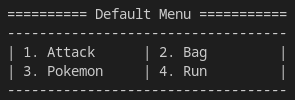
\includegraphics[height=2cm]{media/Menu.png}\end{center}
  
  \section{Unit testing and debugging}
  
  There will be a test log, which will be updated as the project progresses. \par
  We will utilize makefiles to run driver programs to test the classes and also to compile the program. \par 
  Comprehensive testing on edge cases will be done to ensure that the program is robust. 
    
\end{document}
